\documentclass[12pt, twoside]{article}
\usepackage[francais]{babel}
\usepackage[T1]{fontenc}
\usepackage[latin1]{inputenc}
\usepackage[left=6mm, right=6mm, top=6mm, bottom=6mm]{geometry}
\usepackage{float}
\usepackage{graphicx}
\usepackage{array}
\usepackage{multirow}
\usepackage{amsmath,amssymb,mathrsfs}
\usepackage{soul}
\usepackage{textcomp}
\usepackage{eurosym}
 \usepackage{variations}
\usepackage{tabvar}


\pagestyle{empty}

\begin{document}

%4e4

\section*{\center{Devoir maison 4}}

\textit{Devoir � rendre sur feuille grand format petits
carreaux pour le \ul{lundi 01 f�vrier 2010}.}



\subsection*{Exercice 1}

Le stade du Parc des Cygnes peut contenir 15 000 places. Il y a $x$ places en
virage, les autres en tribune. Les places en virage co�tent 10 \euro, les
places en tribune co�tent 13 \euro. Aujourd'hui, le stade est plein.

\begin{enumerate}
  \item Que repr�sentent les trois expressions suivantes:
  
   $10x$ \qquad \qquad  $15 000-x$ \qquad \qquad  $(15 000-x) \times
  13$
  
  \item Ecrire en fonction de $x$ le montant total de la recette (c'est-�-dire
  la somme d'argent gagn�e par la vente des billets.)
  \item Calculer cette recette si x=6500.
\end{enumerate}



\subsection*{Exercice 2}


Sur la figure suivante, AEFG est un carr� de c�t� $x$ et ABCD est un rectangle.

\begin{tabular}{cc}
\begin{minipage}{13cm}


\begin{enumerate}
  \item P�rim�tre de ABCD:
  
  \begin{enumerate}
    \item D�terminer l'expression r�duite donnant le p�rim�tre du rectangle
    ABCD.
    \item Pour x=6cm, calculer le p�rim�tre du rectangle ABCD.
  \end{enumerate}

\item Aire de ABCD:

 \begin{enumerate}
   \item Exprimer l'aire de ABCD sous la forme d'une expression factoris�e.
   \item D�velopper et r�duire l'expression obtenue � la question 2.a)
   \item Pour x=6cm, calculer l'aire du rectangle ABCD de deux fa�ons
   diff�rentes.
 \end{enumerate}
 
\end{enumerate}

\end{minipage}
&
\begin{minipage}{5cm}
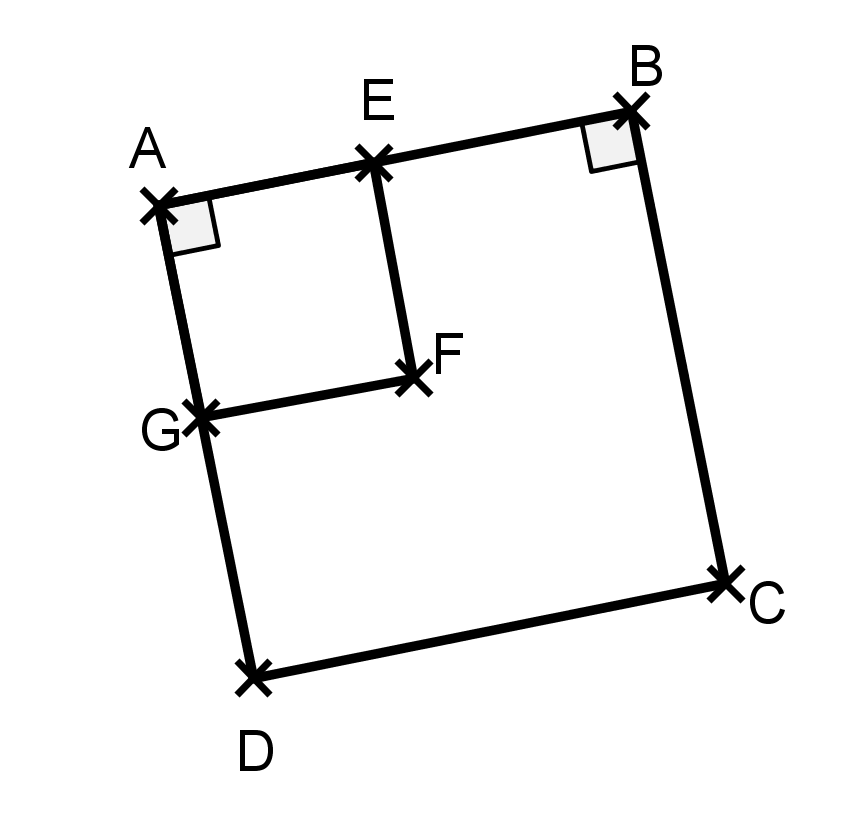
\includegraphics[width=4cm]{images/ex1.png}  
\end{minipage}
\end{tabular}



 

\subsection*{Exercice 3}


R�duire les expressions suivantes:

A=(2x+7)+(3x-6)-(-5-x) \qquad \qquad B=-(5+4y)-(4-4y)+(-3+y)
\qquad \qquad C=3 \big [(x+2)-(3x+5)\big ]






\subsection*{Exercice 4}


On consid�re les expressions D=2x(5x-7)-12(x-1) et E=(2x-4)(-3+5x).

\begin{enumerate}
  \item D�velopper et r�duire les expressions D et E.
  \item Que peut-on en d�duire?
\end{enumerate}

\subsection*{Exercice 5}

Pascal ach�te 7 pains au chocoalt et 4 croissants. un croissant co�te $x$
\euro. Un pain au chocolat co�te 0,20 \euro de plus qu'un croissant.

\begin{enumerate}
  \item Exprimer le prix d'un pain au chocolat en fonction de $x$.
  
  \item  Ecrire en fonction de $x$ la d�pense totale de Pascal.
  \item D�velopper et r�duire l'expression trouv�e.
  \item Si un croissant co�te 0,80 \euro, combien doit payer Pascal?
\end{enumerate}
\end{document}
